\begin{egBox}{Product Topology}[eg:15.1]
    Let us check that the basis given in the [\hyperlink{def:15_product_top}
    {Product Topology Definition}] is indeed a basis. 
    Note that it suffices to only prove for the product between two topological
    spaces since the \( r \)-amount case follows immediately from induction.

    \baseSkip 

    The first condition requires us to show that for each 
    \( ( x, y ) \in X \times Y \), there is at least one basis element 
    containing \( ( x, y ) \);
    this condition is trivially met since \( X \times Y \) is itself a 
    basis element.

    \baseSkip

    The second condition requires us to show that if \( ( x, y ) \) belongs to
    the intersection of two basis elements, say \( U_{ 1 } \times V_{ 1 } \) 
    and \( U_{ 2 } \times V_{ 2 } \), then there is a basis element
    \( U_{ 3 } \times V_{ 3 } \) containing \( ( x, y ) \) such that 
    \( U_{ 3 } \times V_{ 3 } \subset ( U_{ 1 } \times V_{ 1 } )
    \cap ( U_{ 2 } \times V_{ 2 } ) \);
    this condition follows almost immediately since we have that 
    \begin{equation*}
        ( U_{ 1 } \times V_{ 1 } ) \cap ( U_{ 2 } \times V_{ 2 } )
        =
        ( U_{ 1 } \cap U_{ 2 } ) \times ( V_{ 1 } \cap V_{ 2 } )
    \end{equation*}
    Since finite intersections of open sets are open, we have that we can let 
    \( U_{ 3 } = U_{ 1 } \cap U_{ 2 } \) and 
    \( V_{ 3 } = V_{ 1 } \cap V_{ 2 } \), which satisfies the second condition.
\end{egBox}

\begin{egBox}{Standard vs. Product Topology on Euclidean Space}[eg:15.2]
    The set \( \mathbb{R}^{ n } = \mathbb{R} \times \ldots \times \mathbb{R} \)
    has its standard topology induced from the Euclidean metric. 
    This has a basis of open balls.
    Alternatively, we can equip this set with the product topology, where each 
    copy of \( \mathbb{R} \) has been equipped with its standard topology.
    This has a basis of open rectangles.
    We claim that these are the same topologies.

    \baseSkip

    Open balls are open in the product topology since for every point in an arbitrary open ball, we can find some open rectangle contained in the ball that also contains our point.
    Thus, the product topology is at least as fine as the standard topology.
    The same can be said for open rectangles being open in the standard topology
    ; any point in an arbitrary open rectangle is contained within some open
    ball, where the open ball is contained in the open rectangle.
    Thus, the standard topology is at least as fine as the product topology.
    Putting both results together gives us that both topologies are the 
    same.
\end{egBox}

\begin{egBox}{Sorgenfrey Plane}[eg:15.3]
    Let \( \mathbb{R}_{ \ell } \) denote \( \mathbb{R} \) with the lower-limit
    topology.
    The topological space \( \mathbb{R}_{ \ell } \times \mathbb{R}_{ \ell } \)
    is referred to as the \textbf{Sorgenfrey Plane}.
    Let's examine open subsets of the Sorgenfrey plane.

    \begin{figure}[H]
        \centering
        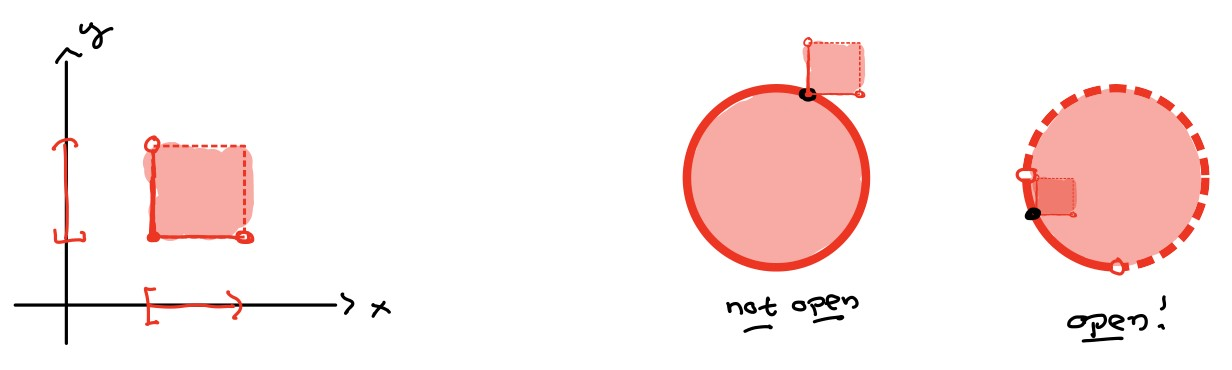
\includegraphics[ width = 0.4\linewidth ]{figures/Section 15/15-3-1.jpg}
        \caption{Open Subsets in the Sorgenfrey plane}
        \label{fig:15-4}
    \end{figure}

    \baseSkip

    Let's examine the subspace topology on the line defined by \( y = x \)
    in \( \mathbb{R}_{ \ell } \times \mathbb{R}_{ \ell } \).
    Something open in this subspace looks like an interval whose lower endpoint 
    is included but the upper endpoint is not -- like a slanted lower limit 
    topology.

    \begin{figure}[H]
        \centering
        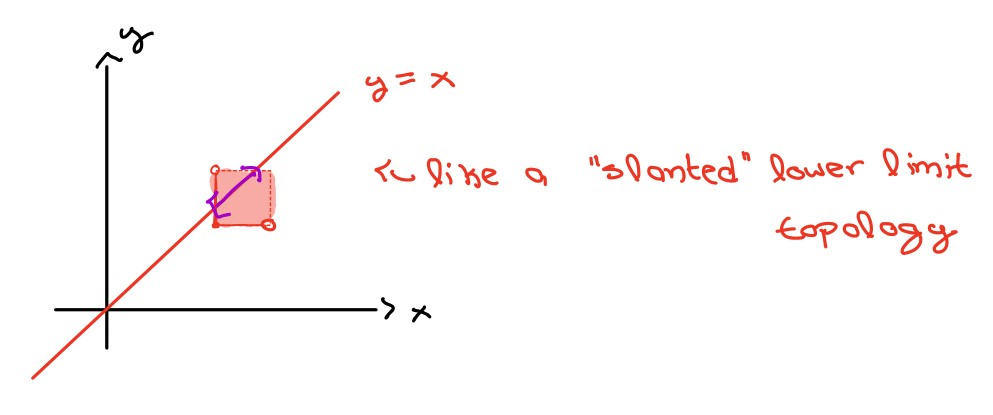
\includegraphics[ width = 0.4\linewidth ]{figures/Section 15/15-3-2.jpg}
        \caption{Subspace topology of \( y = x \)}
        \label{fig:15-5}
    \end{figure}

    \baseSkip 

    Let's examine the line defined by \( y = - x \) in \( \mathbb{R}_{ \ell } 
    \times \mathbb{R}_{ \ell } \).
    In this case, we see that any point on the line is open -- that is, we get 
    a discrete topology.

    \begin{figure}[H]
        \centering
        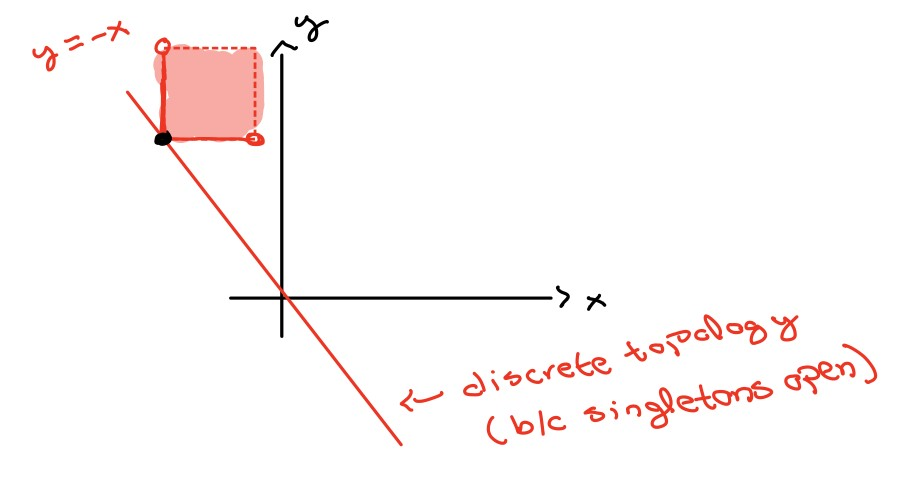
\includegraphics[ width = 0.4\linewidth ]{figures/Section 15/15-3-3.jpg}
        \caption{Subspace topology of \( y = - x \)}
        \label{fig:15-6}
    \end{figure}

    \baseSkip 

    In fact, we see that if the line has a negative slope, then the line 
    inherits the discrete topology;
    when it is positive, we see that the line inherits the lower limit topology.
\end{egBox}
